\section{PSoC Master implementering} \label{sec:PSoC_Master_impl}
Dette afsnit indeholder overvejelser og dokumentation for implementeringen af PSoC Master blokken i systemet.

\begin{figure}[h]
\centering
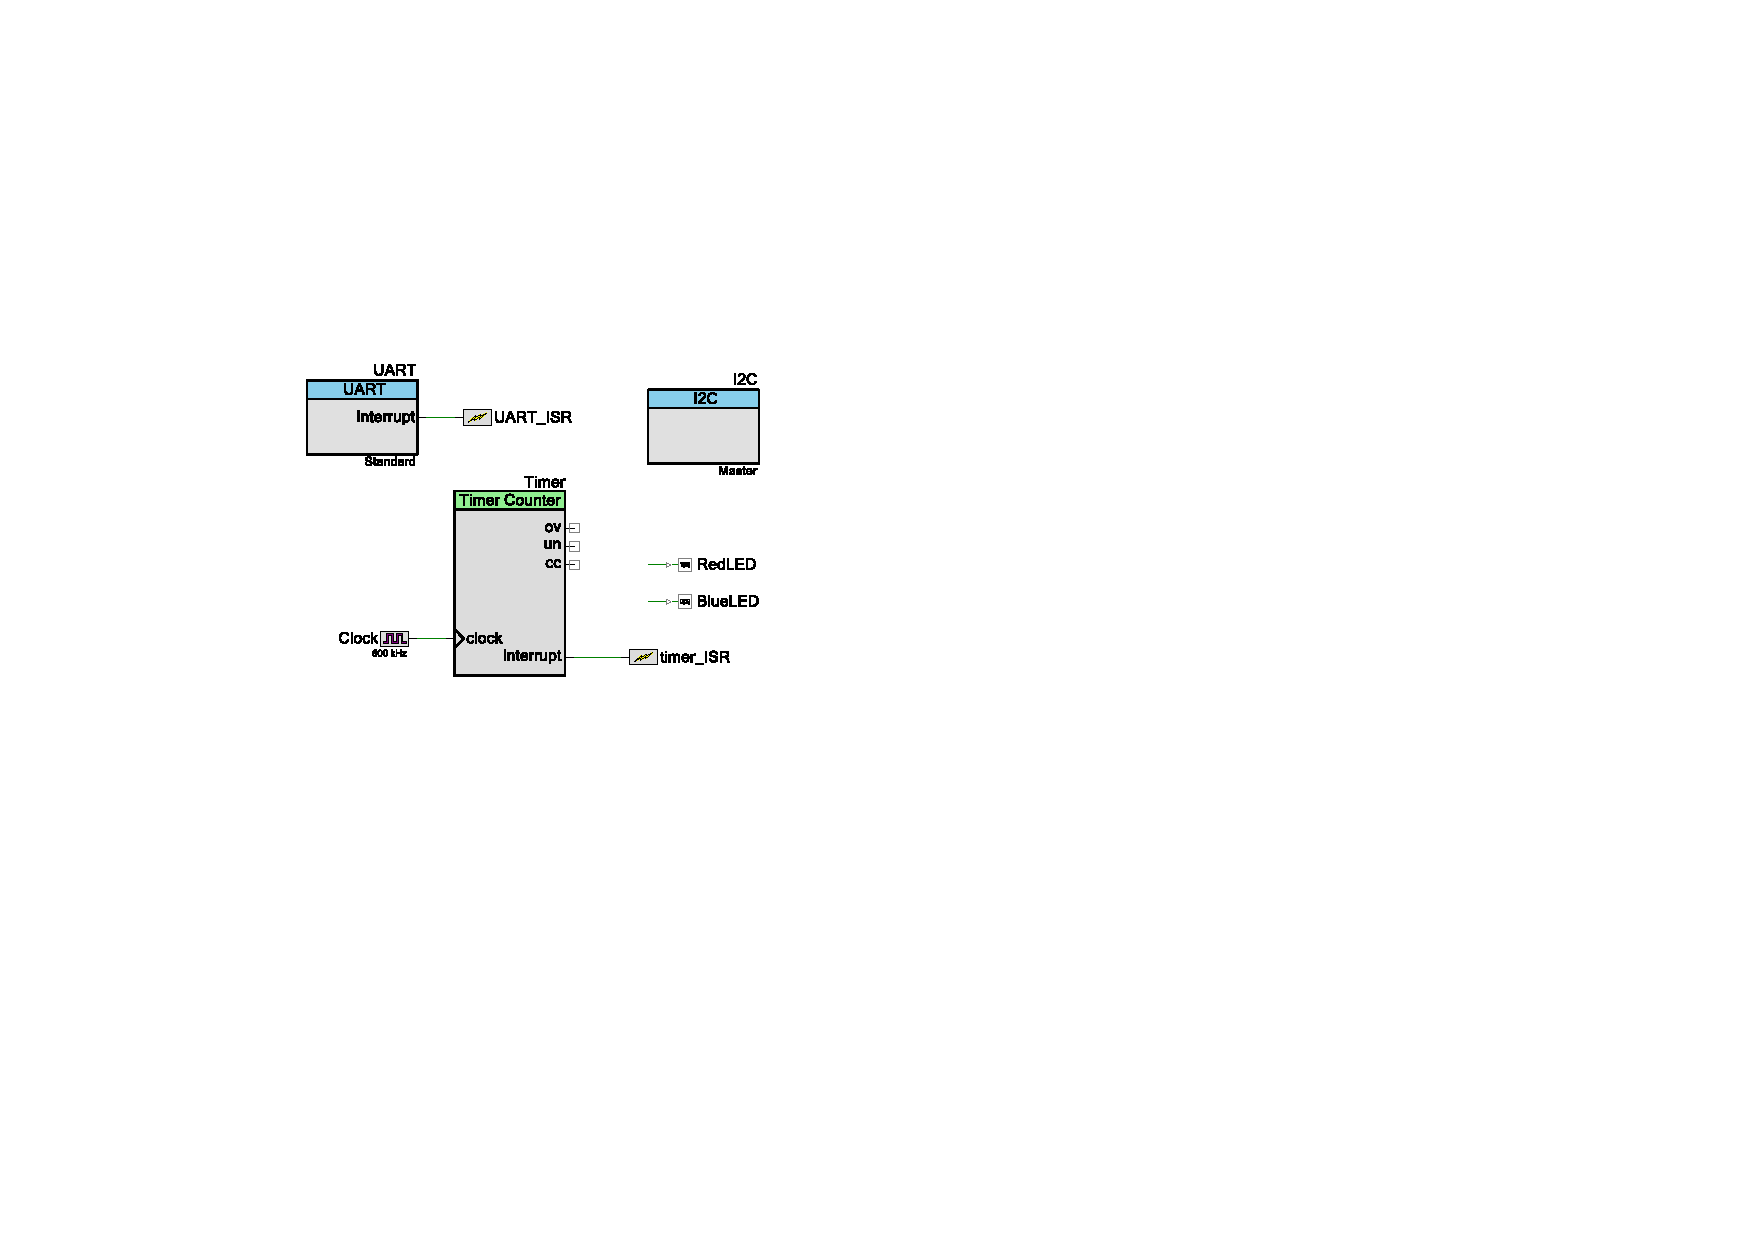
\includegraphics[width=\textwidth*3/5, trim=100 380 500 100, clip=true]{../fig/TopDesign_PSoC_Master}
\label{fig:psoc_master_topdesign}
\caption{TopDesign.cysch for PSoC\_Master}
\end{figure}
  
I Figur \ref{fig:psoc_master_topdesign} ses topdesignet for PSoC Master. Ud fra dette ses det at vi overordnet set har at gøre med en UART, som genererer interrupts, en Timer, som genererer interrupts, en I2C blok og to outputs til LED. 
Selve topdesignet er lavet ud fra de behov der er stillet i Design-fasen. Der blev under implementeringen af UART afprøvet en anden UART komponent grundet problemer med UART kommunikationen, men problemet viste sig at ligge i et tidligere design-valg angående paritet.

\subsection{Main implementering}
Main funktionen, der er vist i Listing \ref{lst:PSoC_Master_main}, er ganske simpel da stort set alt funktionaliteten er håndteret vha interrupts. 
Det er næsten altså kun initialisering af klasserne og efterfølgende konstant kald af to interrupt handler funktioner der finder sted. 
De to funktioner er nærmere beskrevet i afsnittet om Controller klassen på side \pageref{sec:Controller_impl}.

\lstinputlisting[linerange=main0-main1, label=lst:PSoC_Master_main, caption=PSoC Master'ens main funktion]{../src/PSoC_Master/PSoC_Master.cydsn/main.c}

\clearpage

%===================================I2C===================================
\subsection{\IIC implementering} 
I forbindelse med implementeringen af \IIC klassen blev prototyperne oprettet jf. \IIC protokollen (se side \pageref{sec:I2C_protokol}).
Generelt set formidler klassen kald fra både timer og UART og er i stand til at sende og indhente information hhv. fra og til sensorer og aktuatorer der er tilkoblet \IIC-bussen.
Timer klassen anvender \IIC klassen til at hente data fra sensoren med jævne mellemrum.
Dog blev der pga. problemer med de bestilte sensorer ændret i arkitekturen af projektet, hvilket medførte at der anvendes en LM75 i stedet for den tidligere oplyste temperatur/luftfugtsensor.
Ligeledes er lyssensorens implementering nedprioriteret, grundet tidsmangel.

\lstinputlisting[linerange=getTemp0-getTemp1, label=lst:I2C_Class_getTemp(), caption=Implementering af getTemp()]{../src/PSoC_Master/PSoC_Master.cydsn/I2C_Class.c}

I Listing \ref{lst:I2C_Class_getTemp()}, ses der et eksempel på håndtering af en request fra timer interruptet. 
I dette eksempel er det temperatursensoren LM75, der kommunikeres med. 
For at LM75 reagerer på masterens kald, sendes der en slaveadresse og en read-request. 
Denne udskriver to bytes når der læses over \IIC. 
Der sendes herefter en \IIC stop-kommando for at frigøre bussen igen.
Jf. \IIC protokollen på side \pageref{sec:I2C_protokol}, indeholder de to bytes temperaturdata, hvor MSB angiver om temperaturen er negativ eller ej (værdien er signed) og de 8 efterfølgende bits angiver selve temperaturen med en halv grads opløsning. 

Fra aktuatorens side er det valgt, at når der modtages en kommando over \IIC, aktiveres der en interrupt der håndterer den pågældende kommando. 
For \IIC-klassen betyder det at uanset tidspunktet, kan der sendes kommandoer hele tiden, men af hensyn til svaret der skal modtages over bussen, holder masteren klokken lav, indtil enten et svar eller en fejl er modtaget. 
Princippet i read/write funktionen er, at masteren blokerer for andre interrupts og sender en slaveadresse ud på bussen, hvorefter der kommer et acknowledge tilbage fra slaven, som derefter sender et antal bytes ud. 
Det samme kan overordnet siges om write metoden.

\lstinputlisting[linerange=getActuatorStatus0-getActuatorStatus1, label=lst:I2C_Class_getActuatorStatus(), caption=Implementering af getActuatorStatus()]{../src/PSoC_Master/PSoC_Master.cydsn/I2C_Class.c}

Det kan ses på Listing \ref{lst:I2C_Class_getActuatorStatus()} linje 193, at systemet venter på, at bussen bliver ledig. Under debugging af \IIC-klassen var der store problemer, netop med at bussen ikke var ledig under fx. en læsning. 
Problemet viste sig at ligge i rækkefølgen PSoC4 afvikler de interrupts der kommer. 
Systemet ventede med at udføre alle andre metodekald, indtil efter UART'en havde fået et svar. 
Dog udførte systemet stadig en del af funktionaliteten for \IIC read/write, hvilket betød at bussen var optaget i den tid der blev forsøgt at læse. 
Løsningen på problemet viste sig at være en genopbygning af UART- og timer-interruptet, således alt funktionelt blev rykket ud i main og at der bliver sat flag, når det er nødvendigt.

%=================================UART=====================================
\subsection{UART implementering}
UART klassen har til formål at modtage kommandoer fra DevKit8000, tolke disse og give passende svar. 

Generelt set er klassen implementering med udgangspunkt i vores UART protokol, men er udvidet således at der let kan implementeres flere trin i hhv. kontrol af vindue, motor og vanding. UART klassen gør brug af UART komponenten (SCB) vist i Figur \ref{fig:psoc_master_topdesign}.

\lstinputlisting[linerange=respondTemp0-respondTemp1, label=lst:psoc_master_respondTemp, caption=Implementering af respondTemp()]{../src/PSoC_Master/PSoC_Master.cydsn/UART_Class.c}

I Listing \ref{lst:psoc_master_respondTemp} vises et eksempel på en af funktionerne der håndterer svar via UART. De øvrige funktioner i klassen fungerer på samme måde. Funktionen modtager den værdi, der skal sendes tilbage til DevKit8000. Hvis parametren er 0 vil det sige at der er sket en fejl. Når funktionen kaldes kaldes den med returværdi fra DSP klassen, som beskrevet i afsnit \ref{sec:DSP_impl}.

\lstinputlisting[linerange=dkRequest0-dkRequest1, label=lst:psoc_master_dkreq, caption=Implementering af dkRequest()]{../src/PSoC_Master/PSoC_Master.cydsn/UART_Class.c}

Vi har ydermere valgt at indkapsle læsningen fra UART ved hjælp af dkRequest() funktionen vist i Listing \ref{lst:psoc_master_dkreq}. 
Grunden til at vi har valgt at implementere denne er for at sikre os at hvis UART protokollen skulle ændre sig i fremtiden, kan disse ændringer tages højde for i denne funktion inden PSoC Master controllerklassen skal håndtere input fra UART.

Klassen er testet ved at koble en PC på med en COM port og via en terminal indlæse forskellige værdier, for at simulere aktivitet fra DevKit8000. Der er herved kontrolleret at alle muligheder for inputs er tjekket og at klassen udfører det den skal ved hvert input.

%===============================DSP=======================================
\subsection{DSP implementering}\label{sec:DSP_impl}
DSP klassen agerer både digital signal processor og hukommelse for vores måledata. 
Hver type af data er gemt i sit eget array, som vist i Listing \ref{lst:DSP_decl}. 
Hvert arrays har ligeledes en pointer til den næste plads i arrayet der skal overskrives.

\lstinputlisting[linerange=PrivateDataMembers0-PrivateDataMembers1, label=lst:DSP_decl, caption=Deklaration af arrays og pointers]{../src/PSoC_Master/PSoC_Master.cydsn/DSP_Class.c}

Arrays'ne bliver brugt til at gemme en række datapunkter i råt format. Disse datapunkter kan herefter konverteres og midles.
For jordfugt (\texttt{soilHumArray}), er der oprettet et todimensionelt array således at der kan gemmes et array med data for hver af de 6 sensorer.

Når der er målt en ny værdi fra en sensor, via \IIC klassen, bliver den indlæst i DSP klassen med input-funktionerne.

\lstinputlisting[linerange=inputTemp0-inputTemp1, label=lst:DSP_inputTemp, caption=Funktion til at indlæse en sensorværdi i DSP klassen]{../src/PSoC_Master/PSoC_Master.cydsn/DSP_Class.c}

I Listing \ref{lst:DSP_inputTemp} ses \texttt{inputTemp}-funktionen der indlæser den målte værdi i \texttt{tempArray} vha den tilhørende pointer \texttt{tempArrayPtr}. Pointeren flyttes herefter til næste plads i arrayet. Arrayet overskrives på ny når dette er fuldt. Til sidst kaldes den private funktion \texttt{avgTemp}.

\lstinputlisting[linerange=avgTemp0-avgTemp1,label=lst:DSP_avgTemp, caption=Funktion der midler og konverterer tempArray]{../src/PSoC_Master/PSoC_Master.cydsn/DSP_Class.c}

I Listing \ref{lst:DSP_avgTemp} vises avgTemp funktionen. Denne har flere funktionaliteter. Først midles alle de data der er i \texttt{tempArray}, samtidig med at det kontrolleres at der er nok valide datapunkter. Øverst i klassen er der defineret hvor mange valide datapunkter der skal være til stede i et givent array fra en sensor, for at der sendes en værdi videre fra PSoC\_Master til DevKit8000. Herefter konverteres data fra den form det kommer i fra sensorerne, til den form de skal sendes til DevKit8000 i. I dette tilfælde med temperaturen, skal temperaturen begrænses en værdi mellem 1 og 200, jf. UART protokollen som kan ses på side \pageref{sec:UART_protokol}. Når data'en er blevet begrænset, gemmes den i en privat variabel(\texttt{temp}), som herefter kan tilgås med funktionen getTemp\_DSP, der kan ses i Listing \ref{lst:DSP_getTemp}.

\lstinputlisting[linerange=getTemp_DSP0-getTemp_DSP1, label=lst:DSP_getTemp, caption=Getter-funktion som returnerer den seneste midlede temperatur]{../src/PSoC_Master/PSoC_Master.cydsn/DSP_Class.c}

De resterende dele af DSP klassen, altså dem der håndterer jordfugt, luftfugt og lysintensitet, er implementeret efter samme principper og fremgangsmåde og der henvises derfor til kommentarerne i kildekoden som findes i Bilag XXX. for mere information om dette.
%TODO henvisning til kildekodebilag
\clearpage

%===============================PSoC Master===================================
\subsection{Controller implementering} \label{sec:Controller_impl}

PSoC\_Master controller-klassen er som udgangspunkt designet ud fra at blive styret af hvilke kommandoer der er modtaget på UART'en. På den måde agerer vores 'master' slave for DevKit8000. 
For at huske den nuværende status er der oprettet en \texttt{enum} med den nuværende status samt ekstra buffer til at holde styr på hvilken vandingsaktuator der modtages data omkring.

\lstinputlisting[linerange=flags0-flags1, label=lst:PSoC_m_dec, caption=Deklaration af buffers og flag.]{../src/PSoC_Master/PSoC_Master.cydsn/PSoC_Master_Class.c}

Ydermere er der lavet en form for debugging ved hjælp af de tre farvede LED'er på PSoC4 Pioneer Kit. Der tændes fx for den røde LED når et interrupt sker på timeren og for den blå når et interrupt sker på UARTen.

Når der sker et interrupt på UART'en, sættes flaget \texttt{uartInt} til 1 og der fyldes data i bufferen. Dette ses i Listing \ref{lst:PSoC_m_uart_int}.

\lstinputlisting[linerange=UART_ISR0-UART_ISR1, label=lst:PSoC_m_uart_int, caption=ISR for UART.]{../src/PSoC_Master/PSoC_Master.cydsn/PSoC_Master_Class.c}

Årsagen til at vi har valgt at sætte et flag er at vi hurtigst muligt vil ud af interrupt service rutinen samt at det gav os problemer at have al funktionaliteten som kald fra UART ISR.

Der er derfor udarbejdet en ny privat funktion kaldet \texttt{uartIntHandler()}, 
som sørger for at håndtere selve arbejdet mht. det input UART'en giver. 
Denne bliver kaldt med jævne mellemrum fra en \texttt{while(1)} løkke i main.c, se Listing \ref{lst:PSoC_Master_main} på side \pageref{lst:PSoC_Master_main}.

\lstinputlisting[linerange=uartIntHandler0-uartIntHandler1, label=lst:PSoC_m_uartinth, caption=Interrupt handler for UART.]{../src/PSoC_Master/PSoC_Master.cydsn/PSoC_Master_Class.c}

I Listing \ref{lst:PSoC_m_uartinth} ses implementeringen af selve interrupthandleren. Det ses hvordan der først tjekkes for om der er kommet ny data via \texttt{uartInt} og der herefter kontrolleres hvilket stadie, systemet er i. Hvis det er i \texttt{IDLE} tjekkes der på hvad der står i bufferen og der udfærdes evt et svar eller ventes på næste databyte. Til at starte med tændes den blå LED og når kaldet er slut slukkes denne.

Til at indsamle data fra sensorerne med jævne mellemrum er der implementeret en timer med et tilhørende interrupt. 
Denne interrupt service rutine sætter et flag, på samme måde som UART-klassen, som herefter udløser en privat funktion \texttt{timerIntHandler}.

\lstinputlisting[linerange=timerIntHandler0-timerIntHandler1, label=lst:PSoC_m_timerinth, caption=Interrupt handler for timer.]{../src/PSoC_Master/PSoC_Master.cydsn/PSoC_Master_Class.c}

I Listing \ref{lst:PSoC_m_timerinth} ses selve implementeringen af \texttt{timerIntHandler}. 
Den har, ligesom \texttt{uartIntHandler}, en LED der tændes og der udføres herefter selve arbejdet, som består i at fodre data ind i vores digitale signalprocessor (DPS-klassen). 
Data'en kommer fra funktioner i I2C-klassen, der henter selve dataen fra vores sensorer på \IIC bussen.

Værd at notere at for data fra jordfugtsensorerne tjekkes hver sensor for sig, selvom de alle sidder på samme I2C slave reelt set.

\clearpage